% ============================================================
\section{Consequences: partially stable data, equal viscosities and viscous fingering}\label{sec:applications}
% ============================================================

\subsection{Pinch-free data}
\begin{proof}[Proof of Corollary~\ref{cor:pinch}]
If $\Pinch(z_0)=\emptyset$, then $\kmax>0$ on $\T$ and $\kmax\in C^{4,\gamma}(\T)$ (end of Section~\ref{sec:muskat}), so $\kappa:=\theta\kmax$, $\theta\in(0,1)$, satisfies \eqref{eq:kappa-range}, and
Theorem~\ref{thm:A} applies. Conversely, if a single-strip subsolution with opening $\kappa>0$ everywhere exists, Theorem~\ref{thm:B} gives $\kappa\le\kmax$, hence $\kmax>0$ everywhere, i.e.\
$\Pinch(z_0)=\emptyset$. On $\{\sig_0\ge0\}$ the condition $2(1-A\rhom)\kappa<-\sig_0$ of the untilted strip (Remark~\ref{x:rem-normalisations}(a); for $\rhom=A$ it is the range stated in
\cite{LM26}) fails for every $\kappa>0$, so there the admissible opening comes entirely from the term $(1-A^2)\gamma_0^2/(8\mum)$ in $\Phi$, i.e.\ from the vortex sheet.
\end{proof}

For $\rhom=A$ the existence half of Corollary~\ref{cor:pinch} does not need the optimal tilt, and it is latent in \cite{LM26}. With the tilt $\delta_{\rm LM}=-(1-A^2)\gamma_0/(2+A^2)$ of the single
layer of \cite{LM26} (Remarks~\ref{x:rem-normalisations}(b) and~\ref{x:rem-LM26-layer}), the admissible openings are those of \eqref{x:LM-range}, that is, $0<\kappa<\kappa_{\rm LM}$ with
\[
\kappa_{\rm LM}:=\frac{-\sig_0+\sqrt{\sig_0^2+4\delta_{\rm LM}^2}}{4(1-A^2)} ,
\]
the positive root of the quadratic in \eqref{x:LM-range}. It vanishes exactly on $\Pinch(z_0)$. Hence, if $\Pinch(z_0)=\emptyset$, then $\kappa_{\rm LM}\in C^{4,\gamma}(\T)$ is positive, and
Remark~\ref{rem:any-tilt} applies with $\delta=\delta_{\rm LM}$ and $\kappa=\theta\kappa_{\rm LM}$, $\theta\in(0,1)$. In the asymptotically flat setting of \cite{LM26} the same conclusion follows from their
unmodified single layer, once the full modulus $|Au+\ee|$ is kept in the final estimate of \cite[Sec.~7.4]{LM26} and the opening satisfies $c-c_\infty\in H^{k-1}$ and $\inf c>0$
(Section~\ref{x:relation}); \cite{LM26} do not state this. What Corollary~\ref{cor:pinch} adds to \cite{LM26} is the `only if' half (Theorem~\ref{thm:B}); the sharp bound $\kmax\ge\kappa_{\rm LM}$,
whose range improves the coefficient of $\gamma_0^2$ in \eqref{x:LM-range} by the factor $(2+A^2)^2/(4(1+A^2))\in[1,\frac98)$ (Remark~\ref{x:rem-LM26-layer}); an arbitrary intermediate density
$\rhom$; and the periodic setting.

By \eqref{eq:a0} (for $\rhom=A$, cf.\ \cite[(7.11), Prop.~7.4 and (3.7b)]{LM26}), as $\kappa\to0$ the relaxation disc $\{|D-a|<|a|\}$ degenerates only where $\sig_0=\gamma_0=0$; this is the trace on the
interface of the pinch singularity of \cite{Men22} (Remark~\ref{rem:hull}(b)). On the rest of $\Pinch(z_0)$, where $\sig_0>0$ and $\gamma_0=0$, the disc has radius at least $\frac12\sig_0$, but for
every $\kappa>0$ the normal component $D_n=-\sig_0-2(1-A\rhom)\kappa$ of $D$ forced at leading order by the Rankine--Hugoniot conditions lies outside the projection of the disc onto $n_0$: there
$a^{(0)}\cdot\tau_0=0$ and $D_n-2a^{(0)}\cdot n_0=-2(1-A^2)\kappa/\mum<0$ (proof of Lemma~\ref{lem:hull0}).

As in the asymptotically flat setting of \cite{LM26}, where $\sig^{(0)}+2\in H^{k-1}$ \cite[Prop.~6.3]{LM26}, so that $\sig^{(0)}\to-2$ at infinity, our data, which have the heavy fluid on top
($\rho_0=\mathbf 1_{\Omega^+(z_0)}-\mathbf 1_{\Omega^-(z_0)}$), are never fully stable: $\sig_0\ge0$ on all of $\T$ is impossible, because $\int_\T\sig_0\dd s=-4\pi$ (Proposition~\ref{prop:sigma}). This
identity is the periodic counterpart of the normalisation of \cite[Prop.~6.3]{LM26}, and it also follows by integrating $\sig_0=-2(n_{0,2}+AU_0)$, which is \cite[(3.8)]{LM26} in our normalisation, over
a period, since $\int_\T U_0\dd s=0$ (Lemma~\ref{lem:K}(b)). With the heavy fluid below, the integral would be $+4\pi$, and fully stable data exist, for instance the flat interface.

\subsection{Equal viscosities}
\begin{proof}[Proof of Corollary~\ref{cor:A0}]
For $A=0$, Example~\ref{ex:A0} gives $\sig_0=-2n_{0,2}$ and $\gamma_0=-2\tau_{0,2}$ (the formulas of \cite[Secs.~1.2 and~3.1.3]{LM26}), so $\Pinch(z_0)=\{\tau_0=-e_1\}$ and, since
$n_{0,2}^2+\tau_{0,2}^2=1$,
\[
\kmax=\frac{2n_{0,2}+\sqrt{4n_{0,2}^2+4\tau_{0,2}^2}}{4}=\frac{1+n_{0,2}}{2}.
\]
The result follows from Corollary~\ref{cor:pinch} and Theorem~\ref{thm:A}; the regularity of $\kmax$ is clear.
\end{proof}

For $A=0$ the untilted strip ($\delta=0$) has the range $0<\kappa<n_{0,2}$, which is also the range stated in \cite{LM26} ($\bar c<\frac12$, with $c=\kappa$) and only allows mixing where the
interface is a graph. The single layer of \cite{LM26} is, however, tilted: for $A=0$ we have $\delta_{\rm LM}=\delta_*=\tau_{0,2}$, so that at leading order it is exactly the optimally tilted strip.
Moreover, the range of Corollary~\ref{cor:A0} can be read off from \cite{LM26} directly: for $A=0$ we have $|Au+\ee|=1$, and \cite[(7.9)]{LM26} gives $2|\nabla g|=|2\kappa-n_{0,2}|+O(t)$ in their
mixing zone, so that at $t=0$ their exact hull condition \cite[(4.14)]{LM26} reads $|2\kappa-n_{0,2}|<1$, which for $\kappa>0$ means $\kappa<\frac12(1+n_{0,2})$. Turning this into an existence
statement in their setting requires the modification of \cite[Sec.~7.4]{LM26} described in Section~\ref{x:relation}.

The range $0<\kappa<\frac12(1+n_{0,2})$ coincides with $0<\kappa<n_{0,2}$ at horizontal points with the heavy fluid on top ($n_{0,2}=1$). There the total opening speed $2\kappa$ of a single strip is
less than $2$, as for the flat interface, whose single strip with intermediate density $A=0$ has fronts approaching $\pm t$ \cite[Sec.~3.2]{LM26}; this is half of the maximal mixing zone $|x_2|<2t$ of
\cite{Ott99,Sze12} (Example~\ref{ex:flat} with $\theta\to1$). Elsewhere the range is strictly larger. On the overturned part ($n_{0,2}<0$) the tangential component of gravity drives the heavy fluid along
the interface, the interface carries a vortex sheet $\gamma_0=-2\tau_{0,2}\neq0$, and single strips of normal width up to $(1+n_{0,2})t$ are admissible. These are single-strip bounds: for graphs, the
multilayers of \cite[Sec.~7.5]{LM26} give mixing zones of width $4\bar c\,n_{0,2}t$ for every $\bar c<1$, which exceeds $(1+n_{0,2})t$ for $\bar c$ close to $1$ wherever $n_{0,2}>\frac13$. Within
single-strip subsolutions, Theorem~\ref{thm:B} forces the linear opening rate to vanish at the points where the interface is horizontal with the heavy fluid below, and only there; if there is no such
point, every opening $\kappa\in C^{4,\gamma}(\T)$ with $0<\kappa<\frac12(1+n_{0,2})$ is attained (Corollary~\ref{cor:A0}). We prove neither that mixing is impossible near such points nor existence for data
that have them.

For $A=0$, see also \cite{FS18} for stable non-horizontal data and \cite{CFM22} for turned interfaces, where the mixing zone is opened slightly inside the stable regime and, reportedly, the
horizontal stable points (`fully stable points') are identified as an obstruction to mixing; we have not checked this against the full text of \cite{CFM22}, and we have not compared
Corollary~\ref{cor:A0} with their precise admissible ranges. The mixing zones of
\cite{CFM22} for bubbles are localised, and closed bubbles lie outside our horizontally periodic class. Heuristically, for $A=0$ the obstruction of Theorem~\ref{thm:B} also concerns them: a closed $C^1$
curve has a point where the normal pointing into the heavy fluid is $-\ee$, and there a single strip should not open at a positive linear rate. We have not proved a closed-curve analogue of
Theorem~\ref{thm:B}, and for $A\ne0$ the corresponding point need not belong to the analogue of $\Pinch(z_0)$, since $\sig_0$ and $\gamma_0$ are nonlocal. In any case this obstruction is pointwise:
$\kmax=\frac12(1+n_{0,2})>0$ on the rest of the Rayleigh--Taylor stable part, so Theorem~\ref{thm:B} by itself does not force a mixing zone to be localised.

\subsection{Viscous fingering driven by injection}
The original experiments of Saffman and Taylor \cite{ST58} concern a less viscous fluid injected into a more viscous one, without gravity. Consider the problem with gravity constant $G\ge0$ and a uniform
velocity $V\ee$ at infinity:
\begin{equation}\label{eq:IPM-injection}
\partial_t\rho+\dvg(\rho u)=0,\qquad \dvg u=0,\qquad (1+A\rho)u=-\nabla p-G\rho\,\ee,\qquad u(x,t)\to V\ee\ \text{ as }|x_2|\to\infty .
\end{equation}
A weak solution of \eqref{eq:IPM-injection} on $\R^2\times(0,T')$ with initial datum $\rho_0$ is a pair $(\rho,u)\in L^\infty(\R^2\times(0,T'))^{1+2}$ with $\rho^2=1$ a.e.\ which satisfies \eqref{eq:weak}
with $\T\times\R$ replaced by $\R^2$ and $\rho\,\partial_1\varphi$ replaced by $G\rho\,\partial_1\varphi$, and such that $\operatorname{ess\,sup}_{|x_2|>L}|u(x,t)-V\ee|\to0$ as $L\to\infty$ for a.e.\ $t$.
Darcy's law is thus imposed in curl form; since $\R^2$ is simply connected, a pressure can then be recovered distributionally, as in \cite[Sec.~7.4]{LM26}.

\begin{corollary}\label{cor:injection-precise}
Let $G\ge0$, $A\in(-1,1)$ and $V\in\R$ with $G_{\rm eff}:=G+AV>0$. Let $z_0\in\Zc^{6,\gamma}$, $\rhom\in(-1,1)$ and $\kappa\in C^{4,\gamma}(\T)$ with $0<\kappa<\kmax$, where $\kmax$ and $\Pinch(z_0)$ are computed
from $z_0$ and $A$ as in \eqref{eq:Phi} (they do not depend on $G$ and $V$). Let $T$, $Z$ and $z^\pm$ be given by Theorem~\ref{thm:A}. Then there are infinitely many weak solutions of
\eqref{eq:IPM-injection} on $\R^2\times(0,T/G_{\rm eff})$ with initial datum $\mathbf 1_{\Omega^+(z_0)}-\mathbf 1_{\Omega^-(z_0)}$ which are pure outside, and mixing inside, the strip between the curves
\[
z^\pm\big(\cdot,G_{\rm eff}\,t\big)+Vt\,\ee .
\]
In particular, for $G=0$ and $AV>0$ (the displacing fluid is the less viscous one), mixing solutions exist for all pinch-free data.
\end{corollary}

\begin{proof}
Let $(\tilde\rho,\tilde u)$ be one of the solutions given by Theorem~\ref{thm:A}, and set
\[
\rho(x,t):=\tilde\rho\big(x-Vt\ee,\,G_{\rm eff}t\big),\qquad u(x,t):=V\ee+G_{\rm eff}\,\tilde u\big(x-Vt\ee,\,G_{\rm eff}t\big).
\]
For $\varphi\in C^\infty_c(\R^2\times[0,T/G_{\rm eff}))$ let $\psi(y,s):=\varphi\big(y+\frac{Vs}{G_{\rm eff}}\ee,\frac{s}{G_{\rm eff}}\big)$, so that $\psi\in C^\infty_c(\R^2\times[0,T))$,
$\psi(\cdot,0)=\varphi(\cdot,0)$, $G_{\rm eff}\,\partial_s\psi=\partial_t\varphi+V\partial_2\varphi$ and $\nabla_y\psi=\nabla_x\varphi$ at corresponding points. Since $\rho u=V\rho\ee+G_{\rm eff}\tilde\rho\tilde u$,
$(1+A\rho)u+G\rho\ee=V\ee+G_{\rm eff}\big((1+A\tilde\rho)\tilde u+\tilde\rho\ee\big)$, and constant fields integrate to zero against derivatives of test functions, the change of variables
$(y,s)=(x-Vt\ee,G_{\rm eff}t)$, with $\dd x\dd t=G_{\rm eff}^{-1}\dd y\dd s$, turns the three identities of the weak formulation for $(\rho,u)$ and $\varphi$ into those of \eqref{eq:weak}, on $\R^2$, for
$(\tilde\rho,\tilde u)$ and $\psi$. Outside the mixing zone, $\tilde u$ coincides a.e.\ with $\bar u=v/(1\pm A)$ (Theorem~\ref{thm:hprinciple} and \eqref{eq:subsol}), and $v\to\pm\frac{AQ}{4\pi}\ee$ as
$x_2\to\pm\infty$, uniformly in $x_1$ (Lemma~\ref{lem:cauchy}(c) and the proof of Lemma~\ref{lem:mass}), where $Q=0$ because \eqref{eq:mass-cond} holds (Lemmas~\ref{lem:mass} and~\ref{lem:shift}).
Hence $\tilde u\to0$ and $u\to V\ee$. Finally, the affine map $(x,t)\mapsto(x-Vt\ee,G_{\rm eff}t)$ maps open sets to open sets and null sets to null sets, so the solutions are pure outside, and mixing
inside, the preimage of the mixing zone of Theorem~\ref{thm:A}, which is the strip of the statement.
\end{proof}

The physical opening speed of the strip is $G_{\rm eff}\kappa$: $\kmax$ and $\Pinch(z_0)$ refer to the rescaled time $G_{\rm eff}t$. Corollary~\ref{cor:injection-precise} transfers only existence
statements (Theorem~\ref{thm:A}, the `if' part of Corollary~\ref{cor:pinch}, and Corollary~\ref{cor:A0}); we do not transfer Theorem~\ref{thm:B}, which would require replacing condition (S5) of
Definition~\ref{def:single-strip} by $\bar u\to V\ee$ and checking that the change of variables preserves single-strip subsolutions. The hypothesis $G\ge0$ is not used in the proof: $G+AV>0$ suffices,
which also covers a stabilising density contrast ($G<0$) overcome by injection.

Thus injection enters only through the effective gravity $G_{\rm eff}=G+AV$: in the frame moving with the injection, and after rescaling time by $G_{\rm eff}$, the problem is the one studied above. The
condition $G+AV>0$ is the classical Saffman--Taylor criterion for the flat interface \cite{ST58} (see also \cite{Hom87}): a flat interface translating with velocity $V\ee$ has the Saffman--Taylor function
$-2(G+AV)$, as given by $\sig=-2(Gn_2+AU)$, the analogue with gravity constant $G$ of the identity $\sig=-2(n_2+AU)$ of Proposition~\ref{prop:sigma}, i.e.\ of \cite[(3.8)]{LM26}. The rescaling of
time is the normalisation of the gravity constant in \cite[Sec.~1.1]{LM26}. For $G=0$ the instability is purely viscous: in the laboratory frame the Saffman--Taylor function and the vortex-sheet strength
of the data are $AV\sig_0$ and $AV\gamma_0$, with $\sig_0$ and $\gamma_0$ as in \eqref{eq:data}.

The same change of frame applies to any mixing theorem for the normalised problem \eqref{eq:IPM}, in particular to \cite[Thm.~1.1]{LM26} and to the multilayers of \cite[Sec.~7.5]{LM26}: for every
fully unstable datum they give injection-driven mixing solutions, also for fluids of equal density ($G=0$, $AV>0$). Full instability does not depend on the frame, since the Saffman--Taylor function in the
laboratory frame is $G_{\rm eff}\sig_0$. What Corollary~\ref{cor:injection-precise} adds is only the range of Theorem~\ref{thm:A} and the pinch-free data of Corollary~\ref{cor:pinch}. For an optimal bound
on the growth rate of the mixing zone in viscous fingering see \cite{Ott97}.

\subsection{An example}
Let $z_0(\alpha)=(\alpha-1.5\sin\alpha,\ 0.8\sin\alpha)$. Then $\partial_\alpha z_0=(1-1.5\cos\alpha,\ 0.8\cos\alpha)\ne0$, and $z_0$ is injective modulo $2\pi e_1$: if $z_{0,2}(\alpha)=z_{0,2}(\beta)$ with
$\beta\not\equiv\alpha$ then $\beta\equiv\pi-\alpha$ (mod $2\pi$), and $z_{0,1}(\alpha)-z_{0,1}(\pi-\alpha)=2\alpha-\pi$ lies in $2\pi\mathbb Z$ only if $\alpha\equiv\frac\pi2$ (mod $\pi$), in which case
$\beta\equiv\alpha$. Hence $z_0\in\Zc^{k,\gamma}$ for every $k$. The interface is overturned:
$n_{0,2}<0$ for $\cos\alpha>2/3$. The tangent is horizontal only where $\cos\alpha=0$, and there $\tau_0=e_1$. By Corollary~\ref{cor:A0}, for $A=0$ the data are pinch-free although Rayleigh--Taylor
stable on the set $\{\cos\alpha\ge2/3\}$, which makes up $26.8\%$ of the parameter interval and $15.4\%$ of the arclength of one period, and mixing solutions exist with any opening
$\kappa\in C^{4,\gamma}(\T)$ with $0<\kappa<\frac12(1+n_{0,2})$; the minimum of $\frac12(1+n_{0,2})$ is $0.2350$. On the stable set the range stated in \cite{LM26} is empty, whereas for $A=0$ the
range \eqref{x:LM-range} of the single layer of \cite{LM26} with its exact hull condition is that of Corollary~\ref{cor:A0}.

For $A\ne0$ we computed $\sig_0$ and $\gamma_0$ numerically, solving the second kind equations \eqref{eq:data} with the trapezoidal rule on $512$ nodes (the kernel of $\Kop_0$ is smooth). As a
consistency check of this discretisation, identity \eqref{eq:gamma-sigma} (the left relation of \cite[(3.7b)]{LM26} in our normalisation), with $\Top_0$ evaluated by the alternating-point rule, holds
with maximal absolute residual $\le2\cdot10^{-13}$. For $A=0.3$, $-0.6$ and $0.9$ we find $\sig_0\ge0$ on about $26\%$, $24\%$ and $16\%$ of the parameter interval ($15\%$, $14\%$ and $9\%$ of the
arclength), with $\min|\gamma_0|=1.74$, $1.88$ and $2.33$ on that set. Thus the data are pinch-free and partially Saffman--Taylor stable; for $A\ne0$ this is a numerical observation without validated
error bounds (the values above do not change, to the digits given, with $256$ or $1024$ nodes). With $\rhom=A$, the minimum of $\kmax$ over $\T$ is $0.2297$, $0.2265$ and $0.2959$, against $0.2294$,
$0.2224$ and $0.2778$ for the range \eqref{x:LM-range} of the single layer of \cite{LM26} with its exact hull condition, while the range stated in \cite{LM26} is empty on the stable set. The existence
conclusions rely on Theorem~\ref{thm:A}, whose proof is complete modulo the sketches of Appendix~\ref{x:app-sketch}. Figure~\ref{fig:turned} shows the case $A=0.3$. The scripts are in the
\texttt{checks/} folder of the source repository.

\begin{figure}[t]
\centering
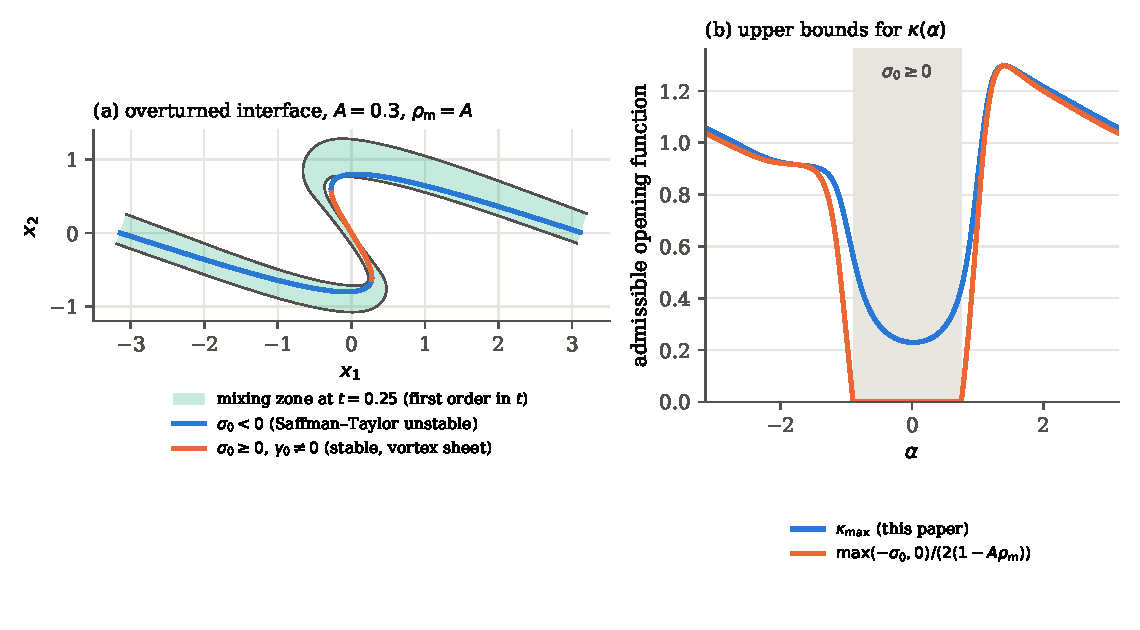
\includegraphics[width=\textwidth]{fig-turned.pdf}
\caption{Overturned interface $z_0(\alpha)=(\alpha-1.5\sin\alpha,0.8\sin\alpha)$ with $A=0.3$ and $\rhom=A$. (a) The initial interface $z_0$, with its Saffman--Taylor stable part $\{\sig_0\ge0\}$
marked in grey, and the strip between $z_0+t(U_0\pm(1\pm\rhom)\kappa)n_0$ for $\kappa=0.8\,\kmax$, i.e.\ the first order part in $t$ of the mixing zone of Theorem~\ref{thm:A}, with its central curve
$z_0+tU_0n_0$. The strip extends along the whole moving interface, including the part where $\sig_0\ge0$; since it is centred on the moving central curve, it does not contain all of $z_0$. The time
$t=0.25$ is illustrative: we have not checked that it is smaller than the existence time $T$ of Theorem~\ref{thm:A}. (b) Single-strip upper bounds for the opening function, as functions of $\alpha$:
$\kmax$ of Theorem~\ref{thm:A}, obtained with the optimal tilt $\delta_*$; the bound $\kappa_{\rm LM}$ of the single layer of \cite{LM26} with its exact hull condition \cite[(4.14)]{LM26}, i.e.\ of the
range \eqref{x:LM-range} (dashed), which differs from $\kmax$ by less than $0.2\%$ for $A=0.3$; and the bound $\max(-\sig_0,0)/(2(1-A^2))$ stated in \cite{LM26} ($\bar c<\frac12$), which is also that of
the untilted strip $\delta=0$ and vanishes on the shaded set $\{\sig_0\ge0\}$.}
\label{fig:turned}
\end{figure}
